% !TeX spellcheck = ru_RU
\documentclass[]{article}

\usepackage{amsmath,amssymb,amsthm,amscd,amsfonts}
\usepackage[utf8]{inputenc}
\usepackage[top=2cm, bottom=2cm]{geometry}
\usepackage{graphicx}
\usepackage[russian]{babel}
\usepackage{xcolor}



\newtheorem{defenition}{Определение}

\begin{document}
	\begin{titlepage}
		\begin{center}
			{\large Федеральное государственное бюджетное образовательное учреждение высшего образования
			<<Санкт-Петербургский Государственный университет>>}
			\vspace{1em}
			
			{\large Кафедра <<Статистического моделирования>>}
			\vspace{18em}
			
			{\bfseries{\Large Отчет по курсовой работе на тему\\ <<Задачи оценивания значимости выравнивания при помощи скрытых марковских моделей>>}}
		\end{center}
		\vspace{10em}
		\begin{flushleft}
			Выполнил:\\
			cт. группы 19.Б04-мм Власенко Даниил Владимирович\\
			Научный руководитель:\\
			к. ф.-м. н. Коробейников Антон Иванович
		\end{flushleft}
		\vspace{20em}
		\begin{center}
			Санкт-Петербург\\
			2021
		\end{center}
	\end{titlepage}

%	\newpage
%	\tableofcontents
%	\newpage
	
	\section{Введение}
		Последовательность длины $L$ "--- строка $D$ состоящая из $L$ символов алфавита $\Sigma$. Выравнивание последовательностей  "--- размещение двух или более последовательностей друг под другом таким образом, чтобы было легче увидеть их схожие участки. Например, даны последовательности ACEAAFAE и CEAFDCE, если расположить их друг под другом, то не будет ни одного совпадения соответствующих символов, но если вставить пропуск восьмого символа в первой последовательности и пропуски первого и пятого символов во второй последовательности, то мы получим 5 совпадений:
		\begin{center}
			\begin{tabular}{ccccccccc}
				A&C&E&A&A&F&A&E\\
				C&E&A&F&D&C&E\\
			\end{tabular}
		\end{center}
		\begin{center}
			\begin{tabular}{ccccccccc}
				A&C&E&A&A&F&A&—&E\\
				—&C&E&A&—&F&D&C&E\\
			\end{tabular}
		\end{center}
		Значимость выравнивания "--- действительное число s, отражающее сходство последовательностей. Способом вычисления значимости выравнивания s может быть, например, увеличение значимости на 1 при совпадении символов, стоящих друг под другом, и уменьшение на $\frac{1}{2}$ при несовпадении. Тогда значимость s приведенного выше выравнивания будет равна 3. Способ вычисления значимости выравнивания выбирается исходя из целей и вида выравнивания.
		
		Сходство последовательностей может отражать функциональные, структурные или эволюционные взаимосвязи объектов, которые описывают эти последовательности. Таким образом вычисление значимости выравнивания последовательностей может быть полезно в задаче определения степени родства биологических организмов путем сравнения их ДНК или РНК, нуклеотидных последовательностей, задаче анализа свойств белков, аминокислотных последовательностей, задаче распознавания речи человека или письменного языка и многих других приложениях.
		
		Выше был приведен пример попарного выравнивания двух строк, но если сходство последовательностей слабое, то через такое выравнивание может не выйти идентифицировать взаимосвязь описываемых последовательностями объектов. Однако сравнение сразу трех и более последовательностей может позволить выявить эту взаимосвязь, такое выравнивание называется множественным. Проводить множественное выравнивание стандартными методами динамического программирования для попарного выравнивания \cite{Compeau15_1} вычислительно неэффективно, но оказывается, что аппарат скрытых марковских моделей (СММ) позволяет эффективно решать эту задачу \cite{Dugad96, Compeau15_2}. 
		
		СММ будут описаны далее, пока что зададимся следующим вопросом. Если есть множество последовательностей, описывающих взаимосвязанные объекты, имеется еще одна последовательность и была посчитана значимость выравнивания этой последовательности ко всему множеству каким-либо способом, то
		\begin{itemize}
			\item достаточно ли высокая эта значимость, чтобы считать объект, описываемый последовательностью, родственным к объектам, описываемым множеством, или шум, т.е. случайная последовательность, мог добиться такой значимости.
			\item достаточно ли низкая эта значимость, чтобы считать объект описываемый последовательностью, не родственным к объектам, описываемым множеством, или сигнал, т.е. последовательность, описывающая взаимосвязанный с множеством объект, мог получить такую значимость. 
		\end{itemize}
		Ложноположительная вероятность значимости s "--- это вероятность того, что шум получит значимость равную или выше s. 
		
		Далее будет описаны метод, который позволяет эффективно вычислять введенный выше термин \cite{Newberg09}.
		
		Исходный код можно изучить на GitHub "--- github.com/Daniil-Vlasenko/SPbUSignificanceEs-\\timation.git.
		
		\section{Метод}
		Сначала опишем модели, затем алгоритмы, которые используются для манипуляции ими.
		\subsection{Модели}
		Метод предполагает, что даны профильная СММ \cite{Compeau15_2}, с помощью которой будут оцениваться последовательности, и фоновая модель $B$, которая будет описывать шум.
		\subsubsection{Скрытые марковские модели}						
			\begin{defenition}
				Пусть $X_{n}$ и $Y_{n}$ дискретные стохастические процессы, $n \geq 1$. Пара $(X_{n}, Y_{n})$ называется скрытой марковской моделью, если
				\begin{itemize}
					\item $X_{n}$~--- марковский процесс, поведение которого напрямую не наблюдается ("скрытый");
					\item $P(Y_{n} = y_{n}|X_{1} = x_{1},\dots, X_{n} = x_{n}) = P(Y_{n}|X_{n}=x_{n})$ для любого $n \geq 1$, где $x_{1},\dots,x_{n}$~--- значения, принимаемые процессом  $X_{n}$ (\textbf{состояния модели}), $ y_{n}$~--- значение, принимаемое процессом $Y_{n}$ (\textbf{наблюдаемый символ модели}).
				\end{itemize}
			\end{defenition}
		
			Примером простой СММ может быть модель, изображенная на рисунке 1 и описывающая подбрасывание двух монет. Пусть между наблюдателем и человеком с монетами стоит ширма, которая позволяет наблюдателю видеть только пол, куда падают монеты. Пусть есть две монеты: одна "--- честная монета, вторая "--- нечестная монета с перевесом в одну из сторон. Пусть человек с монетами с некоторой вероятностью либо подбрасывает монету, которую он бросил в прошлый раз, либо меняет монеты и бросает новую. При этом наблюдатель не знает, какая монета используется в конкретный момент времени, так как он не видит рук бросающего монеты и не может отличить одну монету от другой по их внешнему виду, он видит только последовательность результатов бросков.
			
			\begin{figure}[h]
				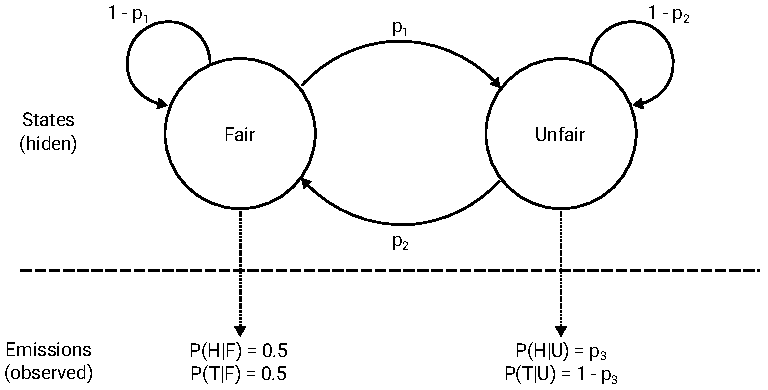
\includegraphics[width=10cm]{figure1}
				\centering
				\caption{Простая скрытая марковская модель.}
			\end{figure}
		
			\subsubsection{Профильная скрытая марковская модель}
			Профильная СММ "--- это СММ со специальной линейной архитектурой состояний, которая позволяет выравнивать последовательность к множеству последовательностей.						
									
			Если для удобства реализации алгоритмов добавить специальное \textit{начальное} и специальное \textit{конечное} состояния, в которых профильная СММ начинает и заканчивает работу и не испускает наблюдаемых символов, как показано на рисунке 2, тогда \textit{путь} $\pi$ в профильной СММ начинается в начальном состоянии, заканчивается в конечном состоянии и проходит от состояния к состоянию, испуская в каждом состоянии наблюдаемый символ, то есть мы считаем, что путь $\pi$ включает в себя и состояния, и наблюдаемые символы. \textit{Последовательность} $D$, связанная с путем $\pi$ "--- последовательность наблюдаемых символов, которая была получена в результате прохода профильной СММ пути $\pi$. 
			
			\begin{figure}[h]
				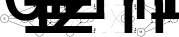
\includegraphics[width=15cm]{figure2}
				\centering
				\caption{Профильная скрытая марковская модель.}
			\end{figure}
			
			\textit{Вероятность пути} $s(\pi)$ "--- произведение всех переходных вероятностей от состояний к состоянию и вероятностей наблюдаемых символов, которые излучаются в каждом состоянии, кроме начального и конечного, на протяжении всего пути $\pi$. 
			
			\textit{Вероятность последовательности} $D$ может интерпретироваться и считаться по-разному "--- алгоритмом \textit{Витерби} или \textit{Форвард} алгоритмом \cite{Dugad96, Compeau15_2}.
			
			Вероятность Витерби $s_{max}(D)$ последовательности $D$ "--- это максимальная вероятность последовательности $D$ среди всех путей $\pi$, которые могли бы ее испустить:
			\begin{equation}
				s_{max}(D) = \underset{\pi \in \pi_{D}}{max}(s(\pi)),
			\end{equation}
			Несмотря на большое количество возможных путей, которые могли бы испустить последовательность $D$, алгоритм Витерби позволяет эффективно решать эту задачу.
			
			Форвард вероятность $s_{fw}(D)$ последовательности $D$ "--- это общая вероятность того, что в результате работы СММ будет получена последовательность $D$:
			\begin{equation}
				s_{fw}(D) = \sum_{\pi \in \pi_{D}}s(\pi).
			\end{equation}
			Форвард алгоритм работает за то же время, что и алгоритм Витерби.
			
			Третий способ оценивать последовательности, позволяющий уменьшить дисперсию дальнейших вычислений оценки ложноположительной вероятности значимости, заключается в том, что каждая вероятность перехода из одного состояния в другое и вероятность излучения символа состоянием будут возводится в степень $\frac{1}{T}$, где $T \in (0; +\infty)$. При этом логика вычислений остается та же, то есть $s(\pi)^{\frac{1}{T}}$ и $s(D)^{\frac{1}{T}}$ будут вычисляться как вероятность произведения независимых событий и как сумма непересекающихся событий соответственно, хотя они уже могут не являться вероятностями (Например, сумма всех $s(\pi)^\frac{1}{T}$ не обязательно равна единице):
			\begin{equation}
				Z(D, T)	= \sum_{\pi \in \pi_{D}}s(\pi)^{\frac{1}{T}}.
			\end{equation}		
			Функция $Z(D, T)$ называется статистической суммой и вычисляется через модификацию Форвард алгоритма. Метод подбора параметра $T$ будет описан далее.
			
			\subsubsection{Фоновая модель}
			Мы предполагаем наличие простой фоновой модели $B$ для последовательностей длины $L$ такой, что все $L$ символьных позиций независимы и одинаково распределены в соответствии с некоторым распределением $Pr(d|B)$, где $d$ отражает возможный наблюдаемый символ:
			\begin{equation}
				Pr(D|B) = \prod_{i=1}^{L}Pr(d_{i}|B),
			\end{equation}
			где $d_{i}$ "--- это $i$-ый наблюдаемый символ последовательности $D$.
			
			\subsection{Постановка математической проблемы}
			Вероятность последовательности $D$ длины $L$ сравнивается с остальными последовательностями той же длины. Определим ложноположительную вероятность значимости:
			\begin{equation}
				fpr(s_{0}) =  \sum_{D \in D_{L}} Pr(D|B) \Theta(s(D) \geq s_{0}),
			\end{equation}
			где $Pr(D|B)$ "--- условная вероятность последовательности $D$, описываемая фоновой моделью, $s(D)$ "--- вероятность последовательности $D$, считаемая профильной СММ, и
			\[
				 \Theta(s(D) \geq s_{0}) = 
				 \begin{cases}
				 	1, & s(D) \geq s_{0}\\
				 	0, & s(D) < s_{0}
				 \end{cases}.
			\]
			То есть $fpr(s_{0})$ "--- это вероятность того, что шум достигнет или превзойдет значимость $s_{0}$. В определении $fpr(s_{0})$ вероятность $D$ отмечена как $s(D)$, потому что способ оценки последовательности может выбираться относительно интересующего приложения, подходит $s(D) = s_{max}(D)$ и $s(D) = s_{fw}(D)$.
			
			\subsection{Алгоритм}
			\subsubsection{Выборка по значимости}
			Так как вычисление $fpr(s_{0})$ через формулу 5 обычно неосуществимо, значение $fpr(s_{0})$ может быть оценено через выборку по значимости, то есть через моделирование строк в соответствии с фоновой моделью $B$ и оценивание значения $fpr(s_{0})$ долей тех из них, что достигают значимости $s_{0}$.
			
			Построим распределение, относительно которого будем моделировать строки. Пусть $P(D|T)$ "--- это условная вероятность строки $D$ относительно некоторой модели строк длины $L$ параметризованной значением $T$. Тогда можно переписать $fpr(s_{0})$:
			\begin{equation}
				fpr(s_{0}) = \sum_{D \in D_{L}} Pr(D|T) f(D,s_{0}),
			\end{equation}
			где
			\begin{equation}
				f(D,s_{0}) = \frac{Pr(D|B) \Theta(s(D) \geq s_{0})}{Pr(D|T)}.
			\end{equation}
			Мы можем оценить значение $fpr(s_{0})$ через моделирование последовательностей в соответствии с этой альтернативной моделью и подсчет среднего значения $f(D,s_{0})$. Этот подход и называется \textit{выборкой по значимости}, он полезен, потому что если правильно подобрать альтернативную модель, то удастся уменьшить дисперсию оценки $fpr(s_{0})$:
			\begin{equation}
				\sum_{D \in D_{L}}Pr(D|T)(f(D, s_{0})-fpr(s_{0}))^{2} <\!\!< \sum_{D \in D_{L}}Pr(D|B)(\Theta(s(D) \geq s_{0})-fpr(s_{0}))^2
			\end{equation}
		
			Определим модель, используемую для выборки по важности параметризованную $T$ следующим образом:
			\begin{equation}
				Pr(D|T) = \frac{P(D|B)Z(D,T)}{Z(T)},
			\end{equation}							
			где 
			\begin{equation}
				Z(T) = \sum_{D \in D_{L}}Pr(D|B)Z(D,T).
			\end{equation}	
			Подставив определение $Pr(D,T)$ в уравнение 7 получим 
			\begin{equation}
				f(D,s_{0}) = \frac{Z(T)\Theta(s(D) \geq s_{0})}{Z(D,T)}.
			\end{equation}		
		
			\subsubsection{Моделирование выборки}
			В итоге мы хотим смоделировать последовательности в соответствии с распределением $Pr(D|T)$, вычислить $f(D, s_{0})$ для каждой последовательности и использовать среднее этих значений как оценку $fpr(s_{0})$. Здесь будет описан метод моделирования последовательностей.
			
			Сначала, используя фоновую модель определенную уравнением 4, вычисляется значение $Z(D)$ через модификацию Форвард алгоритма, вычисляющего $Z(D,T)$. В алгоритме, вычисляющем $Z(D,T)$, излучение символа $d$ некоторым состоянием $E$ связывалось с вероятностью излучения этого символа этим состоянием, возведенной в степень $\frac{1}{T}$ "--- $s_{E}(d)^{\frac{1}{T}}$. В алгоритме вычисляющем $Z(T)$ вместо такого множителя используется среднее значение излучений для состояния $E$:
			\begin{equation}
				\langle s_{E}^{T} \rangle_{B} = \sum_{d'}Pr(d'|B)s_{E}(d)^{\frac{1}{T}}.
			\end{equation}					
			Потому что намного эффективнее заранее вычислить эти значения и хранить их, чем вычислять значение $Z(T)$ напрямую через формулу 10.
			
			Мы моделируем строку длины $L$ обратным ходом по форвард таблице, полученной в результате вычисления $Z(T)$. А точнее мы моделируем путь $\pi$, при этом вероятность излучения состоянием $E$ символа $d'$ следующая:
			\begin{equation}
				Pr_{E}(d') = \frac{Pr(d'|B)s_{E}(d')^{\frac{1}{T}}} {\langle s_{E}^{T} \rangle_{B}}.
			\end{equation}			
			Таким образом мы моделируем путь $\pi$ из распределения 
			\begin{equation}
				Pr(\pi|T) = \frac{Pr(D|B)s(\pi)^{\frac{1}{T}}}{Z(T)}.
			\end{equation}
			Дальше мы оставляем только наблюдаемые символы, забывая состояния, и получаем строку $D$. Так как строка $D$ могла быть излучена разными путями, получаем следующую вероятность моделирования строки $D$ этим методом:
			\begin{equation}				
				Pr(D|T) = \sum_{\pi \in \pi_{D}} \frac{Pr(D|B)s(\pi)^{\frac{1}{T}}}{Z(T)}.
			\end{equation}	
			
			\subsubsection{Оценивание ложноположительной вероятности значимости}			
			Мы хотим оценить ложноположительную вероятность выравнивания для значения $s_{0}$. Для каждой последовательности из $N$ смоделированных последовательностей $\{D_{i}:i=1,\dots,N\}$ мы вычисляем $s(D_{i})$ и $Z(D_{i}, T)$. Тогда оценка $fpr(s_{0})$ следующая:
			\begin{equation}	
				\widehat{fpr(s_{0})} = \frac{Z(T)}{N} \sum_{1}^{N} \frac{\Theta(s(D_{i}) \geq s_{0})}{Z(D_{i}, T)} = 1-\widehat{tpr(s_{0})},
			\end{equation}				
			где $\widehat{tpr(s_{0})}$ оценка истиннонегативной вероятности выравнивания $s_{0}$.
			
			\subsubsection{Выбор T}
			Так как связь между параметром $T$ и значимостью выравнивания $s_{0}$ неявная, то перед осуществлением алгоритма нужно сначала проверить, при каком параметре $T$ оценка $fpr(s_{0})$ имеет меньшую дисперсию. Для этого придется смоделировать несколько строк для разных $T$, и только потом моделировать выборку из $N$ строк с подходящим параметром $T$. На практике было замечена меньшая дисперсия у таких $T$, при которых 20--60$\%$ смоделированных строк удовлетворяют неравенству $s(D) \geq s_{0}$.
			
			\section{Результаты}						
			Для построения профильной СММ необходимо иметь выравнивание последовательностей, которые считаются взаимосвязанными. При этом если в какой-либо колонке встречается большое количество пропусков, то эта колонка с большей вероятностью может не отражать качества, свойственные всему множеству объектов, описываемых последовательностями. Такие колонки отмечаются и обрабатываются особым образом при построении профильной СММ. Долю же пропусков, которая необходима для того, чтобы считать колонку неважной, определяют в зависимости от решаемой задачи. Пусть в нашем случае эта доля будет равна $\frac{2}{5}$.
			
			Будем использовать следующее выравнивание пяти последовательностей:
			\begin{center}
				\begin{tabular}{cccccccccc}
					A&C&D&E&F&\textcolor{gray}{A}&\textcolor{gray}{C}&A&D&F\\
					A&F&D&A&—&\textcolor{gray}{—}&\textcolor{gray}{—}&C&C&F\\
					A&—&—&E&F&\textcolor{gray}{D}&\textcolor{gray}{—}&F&D&C\\
					A&C&A&E&F&\textcolor{gray}{—}&\textcolor{gray}{—}&A&—&C\\
					A&D&D&E&F&\textcolor{gray}{A}&\textcolor{gray}{A}&A&D&F
				\end{tabular}
			\end{center}
			Шестая и седьмая колонки прозрачнее остальных тем самым отмечены как неважные.
			
			Нас интересует значение ложноположительной вероятности значимостей $s_{0}=10^{-3}$, $s_{0}=10^{-6}$ и $s_{0}=10^{-9}$ для строк длины $L=8$.
			
			Для каждого значения было смоделировано 50 последовательностей для различных параметров $T$, чтобы отобрать подходящие значения параметра. Далее для подобранных $T$ для каждого из четырех значений $s_{0}$ была смоделирована выборка из 1000 последовательностей и выполнена оценка $\widehat{fpr(s_{0})}$ через описанный выше алгоритм, в котором за вероятность последовательности $s(D)$ была взята Форвард вероятность $s_{fw}(D)$. Результаты можно наблюдать в таблице, в которой так же указано настоящее значение $fpr(s_0)$, полученное по формуле 5, и доверительный интервал уровня $\gamma = 0.99$:
			\begin{center}
				\begin{tabular}{ccccc}
					$s_{0}$&T&$\widehat{fpr(s_{0})}$&$fpr(s_{0})$&$[c_{1}(\gamma);c_{2}(\gamma)]$  \\ \hline
					$10^{-3}$&1&0.000130127&0.00013312&[0.0000117484; 0.0008517416] \\
					$10^{-6}$&2&0.0105416&0.0102349&[0.0081853; 0.0134781] \\
					$10^{-9}$&3&0.214698&0.21278&[0.20366; 0.22479] \\					
				\end{tabular}
			\end{center}
			Как можно наблюдать чем выше значимость $s_{0}$ тем меньше вероятность того, что шум может достичь такого значения.
			
			\section{Литература}
			\renewcommand{\refname}{}
			\vspace{-25pt}
			\bibliographystyle{ugost2008mod}
			\bibliography{references}
						
\end{document}